% Options for packages loaded elsewhere
\PassOptionsToPackage{unicode}{hyperref}
\PassOptionsToPackage{hyphens}{url}
%
\documentclass[
]{article}
\usepackage{lmodern}
\usepackage{amsmath}
\usepackage{ifxetex,ifluatex}
\ifnum 0\ifxetex 1\fi\ifluatex 1\fi=0 % if pdftex
  \usepackage[T1]{fontenc}
  \usepackage[utf8]{inputenc}
  \usepackage{textcomp} % provide euro and other symbols
  \usepackage{amssymb}
\else % if luatex or xetex
  \usepackage{unicode-math}
  \defaultfontfeatures{Scale=MatchLowercase}
  \defaultfontfeatures[\rmfamily]{Ligatures=TeX,Scale=1}
\fi
% Use upquote if available, for straight quotes in verbatim environments
\IfFileExists{upquote.sty}{\usepackage{upquote}}{}
\IfFileExists{microtype.sty}{% use microtype if available
  \usepackage[]{microtype}
  \UseMicrotypeSet[protrusion]{basicmath} % disable protrusion for tt fonts
}{}
\makeatletter
\@ifundefined{KOMAClassName}{% if non-KOMA class
  \IfFileExists{parskip.sty}{%
    \usepackage{parskip}
  }{% else
    \setlength{\parindent}{0pt}
    \setlength{\parskip}{6pt plus 2pt minus 1pt}}
}{% if KOMA class
  \KOMAoptions{parskip=half}}
\makeatother
\usepackage{xcolor}
\IfFileExists{xurl.sty}{\usepackage{xurl}}{} % add URL line breaks if available
\IfFileExists{bookmark.sty}{\usepackage{bookmark}}{\usepackage{hyperref}}
\hypersetup{
  pdftitle={CPS analysis revision: JSOES and SWFSC datasets},
  hidelinks,
  pdfcreator={LaTeX via pandoc}}
\urlstyle{same} % disable monospaced font for URLs
\usepackage[margin=1in]{geometry}
\usepackage{color}
\usepackage{fancyvrb}
\newcommand{\VerbBar}{|}
\newcommand{\VERB}{\Verb[commandchars=\\\{\}]}
\DefineVerbatimEnvironment{Highlighting}{Verbatim}{commandchars=\\\{\}}
% Add ',fontsize=\small' for more characters per line
\usepackage{framed}
\definecolor{shadecolor}{RGB}{248,248,248}
\newenvironment{Shaded}{\begin{snugshade}}{\end{snugshade}}
\newcommand{\AlertTok}[1]{\textcolor[rgb]{0.94,0.16,0.16}{#1}}
\newcommand{\AnnotationTok}[1]{\textcolor[rgb]{0.56,0.35,0.01}{\textbf{\textit{#1}}}}
\newcommand{\AttributeTok}[1]{\textcolor[rgb]{0.77,0.63,0.00}{#1}}
\newcommand{\BaseNTok}[1]{\textcolor[rgb]{0.00,0.00,0.81}{#1}}
\newcommand{\BuiltInTok}[1]{#1}
\newcommand{\CharTok}[1]{\textcolor[rgb]{0.31,0.60,0.02}{#1}}
\newcommand{\CommentTok}[1]{\textcolor[rgb]{0.56,0.35,0.01}{\textit{#1}}}
\newcommand{\CommentVarTok}[1]{\textcolor[rgb]{0.56,0.35,0.01}{\textbf{\textit{#1}}}}
\newcommand{\ConstantTok}[1]{\textcolor[rgb]{0.00,0.00,0.00}{#1}}
\newcommand{\ControlFlowTok}[1]{\textcolor[rgb]{0.13,0.29,0.53}{\textbf{#1}}}
\newcommand{\DataTypeTok}[1]{\textcolor[rgb]{0.13,0.29,0.53}{#1}}
\newcommand{\DecValTok}[1]{\textcolor[rgb]{0.00,0.00,0.81}{#1}}
\newcommand{\DocumentationTok}[1]{\textcolor[rgb]{0.56,0.35,0.01}{\textbf{\textit{#1}}}}
\newcommand{\ErrorTok}[1]{\textcolor[rgb]{0.64,0.00,0.00}{\textbf{#1}}}
\newcommand{\ExtensionTok}[1]{#1}
\newcommand{\FloatTok}[1]{\textcolor[rgb]{0.00,0.00,0.81}{#1}}
\newcommand{\FunctionTok}[1]{\textcolor[rgb]{0.00,0.00,0.00}{#1}}
\newcommand{\ImportTok}[1]{#1}
\newcommand{\InformationTok}[1]{\textcolor[rgb]{0.56,0.35,0.01}{\textbf{\textit{#1}}}}
\newcommand{\KeywordTok}[1]{\textcolor[rgb]{0.13,0.29,0.53}{\textbf{#1}}}
\newcommand{\NormalTok}[1]{#1}
\newcommand{\OperatorTok}[1]{\textcolor[rgb]{0.81,0.36,0.00}{\textbf{#1}}}
\newcommand{\OtherTok}[1]{\textcolor[rgb]{0.56,0.35,0.01}{#1}}
\newcommand{\PreprocessorTok}[1]{\textcolor[rgb]{0.56,0.35,0.01}{\textit{#1}}}
\newcommand{\RegionMarkerTok}[1]{#1}
\newcommand{\SpecialCharTok}[1]{\textcolor[rgb]{0.00,0.00,0.00}{#1}}
\newcommand{\SpecialStringTok}[1]{\textcolor[rgb]{0.31,0.60,0.02}{#1}}
\newcommand{\StringTok}[1]{\textcolor[rgb]{0.31,0.60,0.02}{#1}}
\newcommand{\VariableTok}[1]{\textcolor[rgb]{0.00,0.00,0.00}{#1}}
\newcommand{\VerbatimStringTok}[1]{\textcolor[rgb]{0.31,0.60,0.02}{#1}}
\newcommand{\WarningTok}[1]{\textcolor[rgb]{0.56,0.35,0.01}{\textbf{\textit{#1}}}}
\usepackage{graphicx}
\makeatletter
\def\maxwidth{\ifdim\Gin@nat@width>\linewidth\linewidth\else\Gin@nat@width\fi}
\def\maxheight{\ifdim\Gin@nat@height>\textheight\textheight\else\Gin@nat@height\fi}
\makeatother
% Scale images if necessary, so that they will not overflow the page
% margins by default, and it is still possible to overwrite the defaults
% using explicit options in \includegraphics[width, height, ...]{}
\setkeys{Gin}{width=\maxwidth,height=\maxheight,keepaspectratio}
% Set default figure placement to htbp
\makeatletter
\def\fps@figure{htbp}
\makeatother
\setlength{\emergencystretch}{3em} % prevent overfull lines
\providecommand{\tightlist}{%
  \setlength{\itemsep}{0pt}\setlength{\parskip}{0pt}}
\setcounter{secnumdepth}{-\maxdimen} % remove section numbering
\usepackage{booktabs}
\usepackage{longtable}
\usepackage{array}
\usepackage{multirow}
\usepackage{wrapfig}
\usepackage{float}
\usepackage{colortbl}
\usepackage{pdflscape}
\usepackage{tabu}
\usepackage{threeparttable}
\usepackage{threeparttablex}
\usepackage[normalem]{ulem}
\usepackage{makecell}
\usepackage{xcolor}
\ifluatex
  \usepackage{selnolig}  % disable illegal ligatures
\fi

\title{CPS analysis revision: JSOES and SWFSC datasets}
\author{}
\date{\vspace{-2.5em}}

\begin{document}
\maketitle

\hypertarget{data-wrangling}{%
\subsection{Data wrangling}\label{data-wrangling}}

SWFSC data: For these data we removed all night tows (n = 5) and samples
using the fine mesh liner (n = 32). These conditions generally only
affected sampling in 2016 with 2 of the night tows occurring in 2015. We
also removed tows that occurred in August (n = 5) as these samples only
occurred in 2015. The remaining dataset (n = 518) represents samples
that occurred in June, July and September in 2010-2016.

JSOES data: For these data we Cheryl's advice and guidance as to what we
included/excluded in the analysis. Major exclusions included reducing
May samples to the years 1999, 2006-2012. We also excluded any tow where
Study Type did not equal ``regular''. We also removed all samples that
occurred at night (n = 31).

\begin{Shaded}
\begin{Highlighting}[]
\NormalTok{shelf }\SpecialCharTok{\%\textgreater{}\%}
  \FunctionTok{group\_by}\NormalTok{(Study,Year,Month) }\SpecialCharTok{\%\textgreater{}\%}
  \FunctionTok{summarize}\NormalTok{(}\AttributeTok{count=}\FunctionTok{n}\NormalTok{()) }\SpecialCharTok{\%\textgreater{}\%}
  \FunctionTok{kbl}\NormalTok{() }\SpecialCharTok{\%\textgreater{}\%}
  \FunctionTok{kable\_styling}\NormalTok{()}
\end{Highlighting}
\end{Shaded}

\begin{table}
\centering
\begin{tabular}[t]{l|l|l|r}
\hline
Study & Year & Month & count\\
\hline
JSOES & 1998 & June & 35\\
\hline
JSOES & 1998 & September & 35\\
\hline
JSOES & 1999 & June & 23\\
\hline
JSOES & 1999 & May & 9\\
\hline
JSOES & 1999 & September & 43\\
\hline
JSOES & 2000 & June & 22\\
\hline
JSOES & 2000 & September & 17\\
\hline
JSOES & 2001 & June & 42\\
\hline
JSOES & 2001 & September & 40\\
\hline
JSOES & 2002 & June & 35\\
\hline
JSOES & 2002 & September & 38\\
\hline
JSOES & 2003 & June & 49\\
\hline
JSOES & 2003 & September & 34\\
\hline
JSOES & 2004 & June & 45\\
\hline
JSOES & 2004 & September & 29\\
\hline
JSOES & 2005 & August & 24\\
\hline
JSOES & 2005 & June & 19\\
\hline
JSOES & 2005 & September & 39\\
\hline
JSOES & 2006 & June & 44\\
\hline
JSOES & 2006 & May & 21\\
\hline
JSOES & 2006 & September & 53\\
\hline
JSOES & 2007 & June & 44\\
\hline
JSOES & 2007 & May & 37\\
\hline
JSOES & 2007 & September & 34\\
\hline
JSOES & 2008 & June & 36\\
\hline
JSOES & 2008 & May & 29\\
\hline
JSOES & 2008 & September & 43\\
\hline
JSOES & 2009 & June & 36\\
\hline
JSOES & 2009 & May & 27\\
\hline
JSOES & 2009 & September & 31\\
\hline
JSOES & 2010 & June & 41\\
\hline
JSOES & 2010 & May & 23\\
\hline
JSOES & 2010 & September & 26\\
\hline
JSOES & 2011 & June & 37\\
\hline
JSOES & 2011 & May & 28\\
\hline
JSOES & 2011 & September & 31\\
\hline
JSOES & 2012 & June & 30\\
\hline
JSOES & 2012 & May & 16\\
\hline
JSOES & 2012 & September & 35\\
\hline
JSOES & 2013 & June & 27\\
\hline
JSOES & 2014 & June & 40\\
\hline
JSOES & 2015 & June & 40\\
\hline
JSOES & 2016 & June & 41\\
\hline
JSOES & 2017 & June & 37\\
\hline
JSOES & 2018 & June & 43\\
\hline
JSOES & 2019 & June & 47\\
\hline
SWFSC & 2010 & July & 21\\
\hline
SWFSC & 2011 & July & 38\\
\hline
SWFSC & 2011 & June & 6\\
\hline
SWFSC & 2011 & September & 26\\
\hline
SWFSC & 2012 & June & 13\\
\hline
SWFSC & 2013 & July & 6\\
\hline
SWFSC & 2014 & July & 1\\
\hline
SWFSC & 2015 & August & 7\\
\hline
SWFSC & 2015 & July & 6\\
\hline
SWFSC & 2015 & June & 14\\
\hline
SWFSC & 2015 & September & 36\\
\hline
SWFSC & 2016 & July & 3\\
\hline
SWFSC & 2016 & June & 24\\
\hline
\end{tabular}
\end{table}

Next, we z-scored all the coavariates such that mean = 0 and sd = 1
given the the vastly different units of each individual covariate.

We can then look at potential correlations between the covaraites and
for the most part don't see anything that would be a red flag

\begin{Shaded}
\begin{Highlighting}[]
\FunctionTok{ggpairs}\NormalTok{(shelf[,}\FunctionTok{c}\NormalTok{(}\StringTok{"ztemp"}\NormalTok{,}\StringTok{"zsal"}\NormalTok{,}\StringTok{"zlat"}\NormalTok{,}\StringTok{"zDTS"}\NormalTok{)])}
\end{Highlighting}
\end{Shaded}

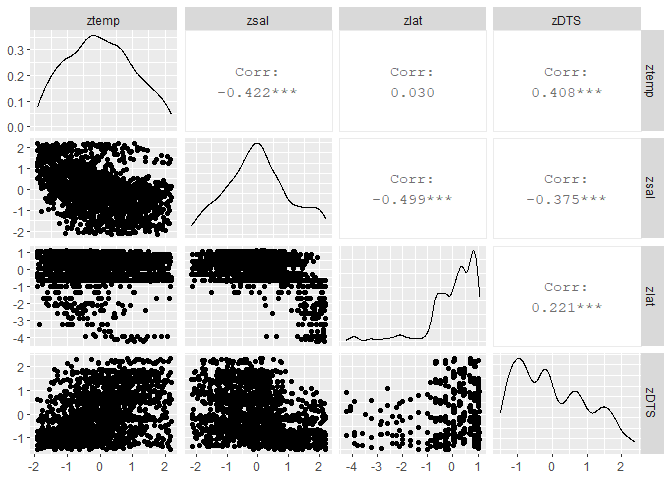
\includegraphics{CPSrevision_files/figure-latex/unnamed-chunk-4-1.pdf}

We can also look at the range and mean of temp and salinity across the
dataset. Both seem pretty stable until we hit 2015 and then things get a
bit less so. Salnity, in partiuclar, looks to be relatively high in 2015
and 2019. Or at least measurements do not indicate salinity in the lower
range of previous years.

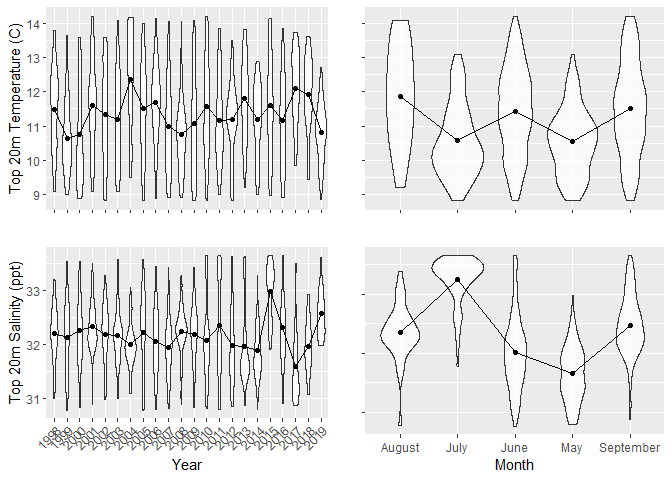
\includegraphics{CPSrevision_files/figure-latex/unnamed-chunk-5-1.pdf}

\hypertarget{analysis}{%
\subsection{Analysis}\label{analysis}}

The major change to our analysis is the inclusion of some temporal
interactions for each covariate. Essentially looking at how any observed
relationship between species P/A and our covariates change as a function
of month. SO we have now added a Month x covariate interaction to each
model.We included all first order interactions with Month and use model
selection to determine the best overall combination for predicting P/A
for each species. We then plot the interactions with significant terms.
Northern Anchovy example below.

\hypertarget{northern-anchovy}{%
\subsubsection{\texorpdfstring{\emph{Northern
Anchovy}}{Northern Anchovy}}\label{northern-anchovy}}

There were 5 models with equal support (AICc) but model weights ranged
from 0.092 to 0.247. All the top models included month, latitude, and
salinity and some combination of interactions with month. The ``best''
model included all the covariates but only the interactions between
months for latitude and distance to shore.

\begin{verbatim}
## Warning in checkConv(attr(opt, "derivs"), opt$par, ctrl = control$checkConv, :
## unable to evaluate scaled gradient
\end{verbatim}

\begin{verbatim}
## Warning in checkConv(attr(opt, "derivs"), opt$par, ctrl = control$checkConv, :
## Model failed to converge: degenerate Hessian with 1 negative eigenvalues
\end{verbatim}

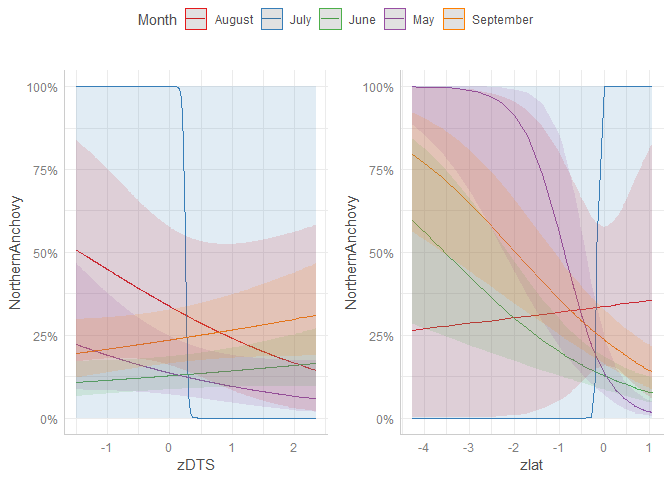
\includegraphics{CPSrevision_files/figure-latex/unnamed-chunk-6-1.pdf}
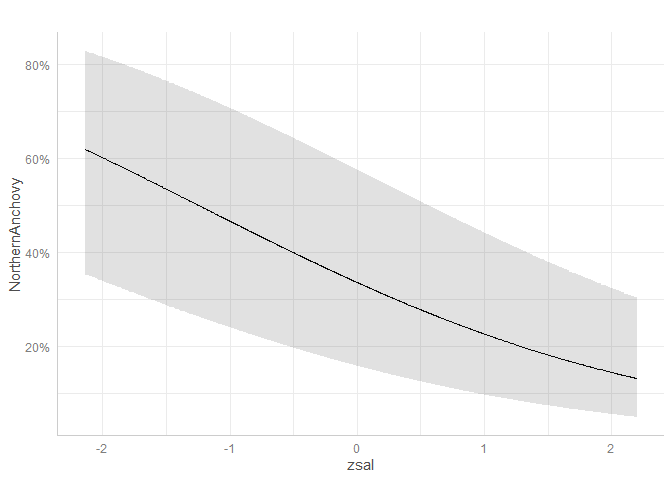
\includegraphics{CPSrevision_files/figure-latex/unnamed-chunk-6-2.pdf}

\hypertarget{pacific-sardine}{%
\subsubsection{\texorpdfstring{\emph{Pacific
Sardine}}{Pacific Sardine}}\label{pacific-sardine}}

The best models did not include interactions between month and other
covaraiates and the best model only includes MOnth, Salinity and
distance to shore. Other models supported by AICc but with lower
relative model weights included either latitude or temperature.

\begin{verbatim}
## Data were 'prettified'. Consider using `terms="zsal [all]"` to get smooth plots.
\end{verbatim}

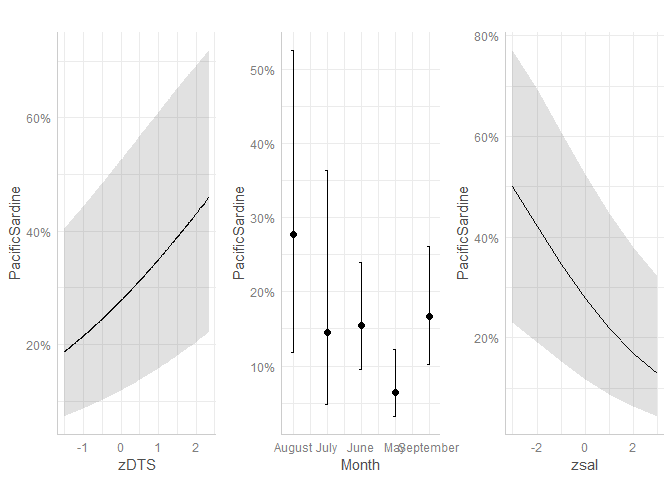
\includegraphics{CPSrevision_files/figure-latex/unnamed-chunk-7-1.pdf}

\hypertarget{market-squid}{%
\subsubsection{\texorpdfstring{\emph{Market
Squid}}{Market Squid}}\label{market-squid}}

All terms were included in the best model with the exception of the
interaction between month and distance to shore. Best model was
overwhelmingly supported over other iterations.

\begin{verbatim}
## Warning in checkConv(attr(opt, "derivs"), opt$par, ctrl = control$checkConv, :
## Model failed to converge with max|grad| = 0.0102755 (tol = 0.001, component 1)
\end{verbatim}

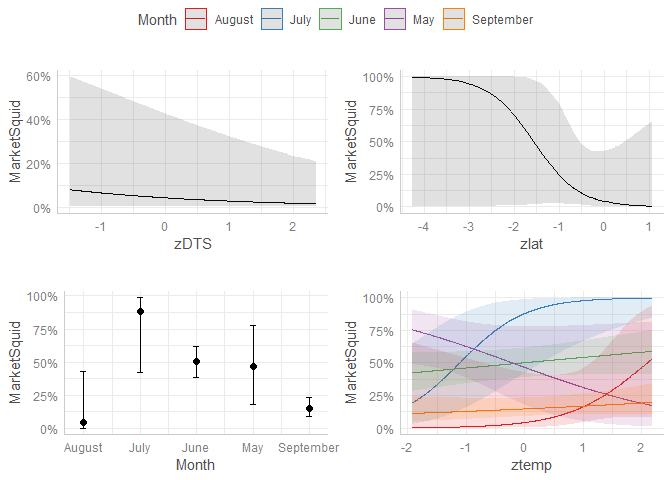
\includegraphics{CPSrevision_files/figure-latex/unnamed-chunk-8-1.pdf}

\hypertarget{pacific-mackerel}{%
\subsubsection{\texorpdfstring{\emph{Pacific
Mackerel}}{Pacific Mackerel}}\label{pacific-mackerel}}

Pacific mackerel only occurred in 3\% of tows for the shelf surveys. Our
analysis suggested that the best fit model include only distance
offshore and temperature with no variation by month. Both showed a
positive effect on presence of Pacific mackerel indicating higher
presence in warmer waters farther offshore. However, while the effect
for distance offshore and temperature nearly doubled the predicted
probability of presence, the predictions remained low (\textless{} 5\%).
Given low presence we should interpret these results with caution.

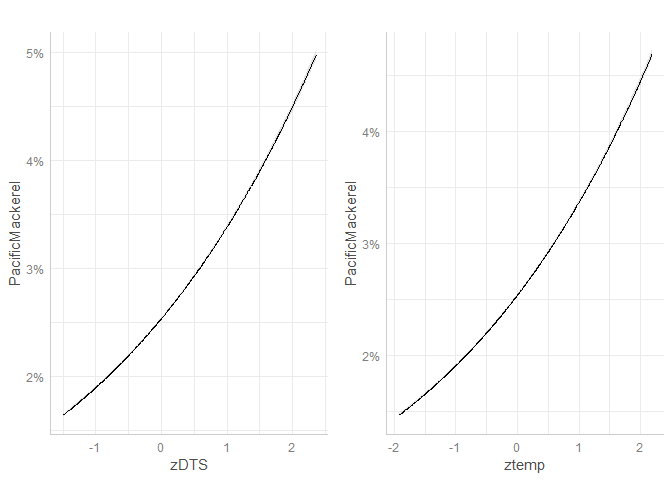
\includegraphics{CPSrevision_files/figure-latex/unnamed-chunk-9-1.pdf}

\hypertarget{jack-mackerel}{%
\subsubsection{\texorpdfstring{\emph{Jack
Mackerel}}{Jack Mackerel}}\label{jack-mackerel}}

Jack mackerel were encountered relatively infrequently (8\%) in the
shelf survey. The best model for predciitng Jack mackerel present in the
shelf survey included all of our covariates as well as their
interactions with month with the exception of the month x distance to
shore effect. Distance to shore was the only significant, albeit very
weak, effect on Jack mackerel presence. There was considerable
variability in Jack mackerel presence by month with low (\textless{}
10\%) predicted probability of presence in all months except July
(\textasciitilde70\%). Model predcitions of presence in July is a severe
over-prediction for Jack Mackerel

\includegraphics{CPSrevision_files/figure-latex/unnamed-chunk-10-1.pdf}
\#\#\# \emph{Pacific Herring}

Herring were not included in the original analysis but i looked at them
here out of my own interest.All terms were included in the best model
with the exception of the interaction between month and temperature.
Models that included the interaction or excluded all temperature terms
were equally supported via AICc but had a slightly lower model weight
than the best fit model. Both salinity and distance offshore were strong
predictors of herring presence. The relationship with distance offshore
differed in magnitude by month bu maintained a negative relationship
indicting herring presence higher closer to shore. Herring presence was
higher in lower salinity in June and July while the opposite was true in
May.

\begin{verbatim}
## Warning in checkConv(attr(opt, "derivs"), opt$par, ctrl = control$checkConv, :
## Model failed to converge with max|grad| = 0.0185599 (tol = 0.001, component 1)
\end{verbatim}

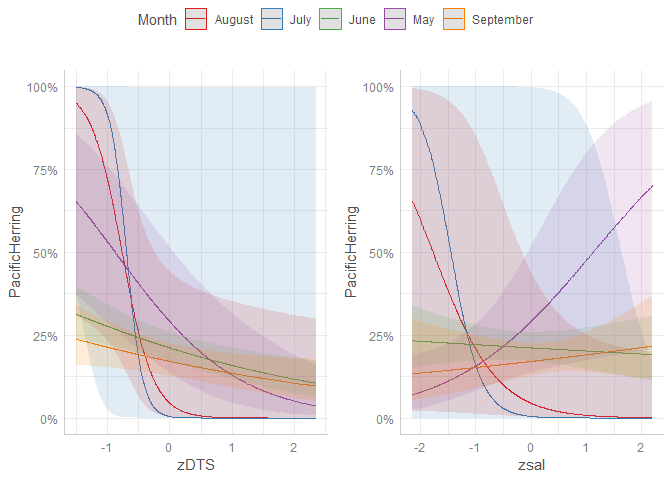
\includegraphics{CPSrevision_files/figure-latex/unnamed-chunk-11-1.pdf}

\hypertarget{revised-results}{%
\subsection{Revised Results}\label{revised-results}}

In general, across all species we analyzed, accounting for temporal
variation in our covariates appears to be informative and provides some
additional information with respect to presence/absence of coastal
pelagic species. INteractions with month we largely driven by
differences associated with July when salinity was generally higher than
other months and the occurrence of CPS in each survey was rather low.

Northern Anchovy occurred in 58\% of Predator survey samples and 19\% of
the Shelf survey samples. Our initial report that combined the Predator
survey data with the ocean ecology surveys found significant effects of
salinity and latitude suggesting increased presence of northern anchovy
with below average salinity (\textasciitilde29ppt) and peak presence
(quadratic shape) occurring at 43.5 N latitude. When we separate the
data out by survey we see similar patterns but with additional
nuances.In both surveys the effect of salinity was negative although
apparently stronger in the predator survey data. The difference in
magnitude may be due to the minimum salinities that were encounter in
each survey (predator = 22.1 ppt, Shelf = 30.2), the predator survey
having sampled less salty water (CR plume).

\begin{figure}
\centering
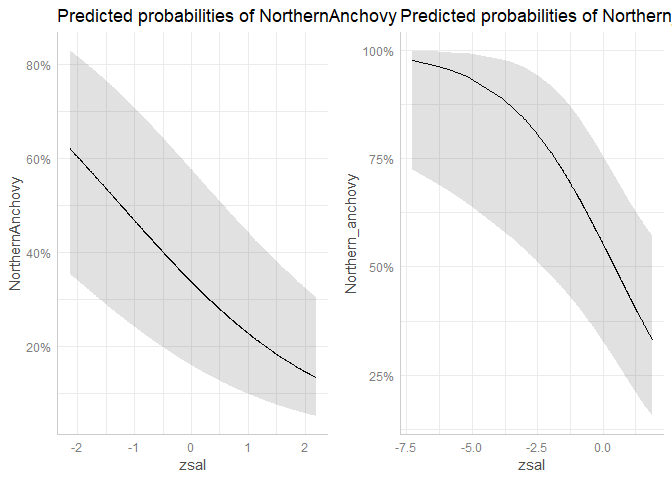
\includegraphics{CPSrevision_files/figure-latex/unnamed-chunk-12-1.pdf}
\caption{Effect of salinity on presence of Northern Anchovy is the
Predator (plume) survey (left)and Shefl surveys (right).}
\end{figure}

Latitude was also important for determining presence/absence of Northern
Anchovy in both datasets. For the Predator dataset Latitude was reduced
to a factor (above and below CR plume) given the lack of variability in
individual station latitudes.Northern anchovy decreased steadily from
May to August above and below the plume with the exception of low
presence in June above the mouth of the CR. For the shelf surveys
Northern anchovy presence was higher at more southern latitudes and this
was true in all months except July and August when Northern Anchovy were
generally absent from the majority of sites across the survey.

\begin{figure}
\centering
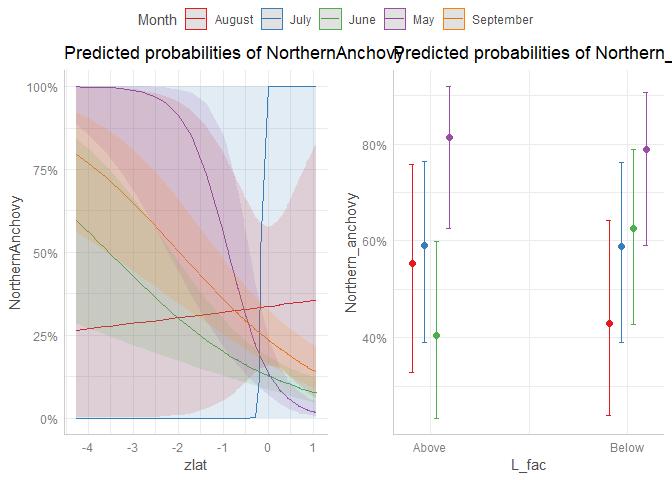
\includegraphics{CPSrevision_files/figure-latex/unnamed-chunk-13-1.pdf}
\caption{Effect of Latitude on presence of Northern Anchovy is the
Predator (plume) survey (left)and Shefl surveys (right).}
\end{figure}

Lastly, although distance to shore was important for determining
Northern Anchovy presence in both survey datasets, the interaction with
month was not consistent among surveys. In general, Northern Anchovy had
a higher probability of presence when samples were taken further
inshore.The effect was considerable in May and June for the Predator
survey. Distance to shore had a somewhat weaker effect on anchovy
presence in the shelf dataset though it was only evident in May and
August and actually showed the opposite trend during September.

\begin{figure}
\centering
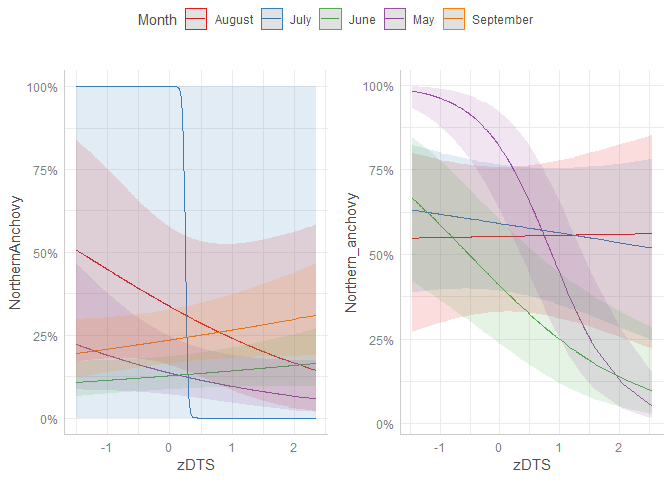
\includegraphics{CPSrevision_files/figure-latex/unnamed-chunk-14-1.pdf}
\caption{Probability of presence of Northern Anchovy as a function of
distance from shoreline for Ocean (left) and Plume (right) surveys.}
\end{figure}

\hypertarget{pacific-sardine-1}{%
\subsubsection{Pacific Sardine}\label{pacific-sardine-1}}

Pacific sardine were encountered in nearly identical proportions to
Northern Anchovy across each survey (52\% and 19\% Predator and shelf
surveys, respectively). Our initial analysis indicated temperature and
latitude had a slightly positive effect on predicted probability of
Pacific Sardine presence and a negative effect of both salinity and
distance offshore. OUr revised analysis generally suggested similar
patterns when the surveys were split although the effect of latitude was
only observed for the predator survey indicating a higher predicted
presence above the Columbia R than below adn termperature only in the
predaotr survey indicating . Therefore our initial interpretations
regarding Pacifc Sardine presence remained largely the same.

Across both surveys presence of Pacific Sardine was predicted to be
relatively low in May compared to other months sampled. Distance
offshore was also positively related to Pacific Sardine presence
indicating sardine were more likely to be encountered the farther
offshore the sample occurred. However, the pattern was reversed in May
for the predator survey potentially indicating a more shoreline oriented
distribution of pacific sardine during this time period.

\begin{figure}
\centering
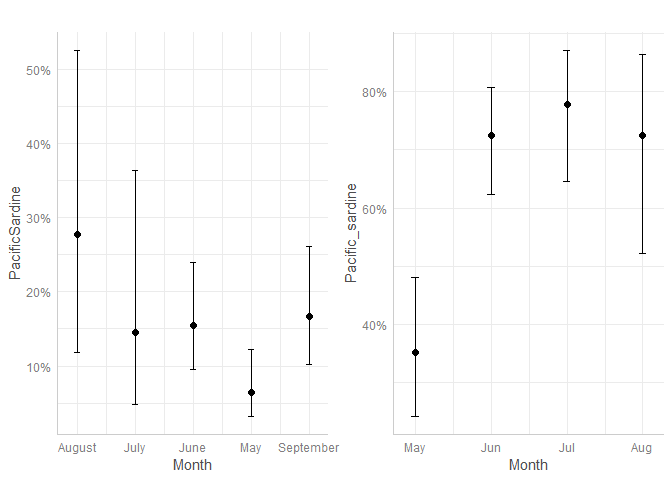
\includegraphics{CPSrevision_files/figure-latex/unnamed-chunk-15-1.pdf}
\caption{predicted probability of Pacific Sardine presence across months
for Shelf (left) and Predator (right) surveys.}
\end{figure}

\begin{figure}
\centering
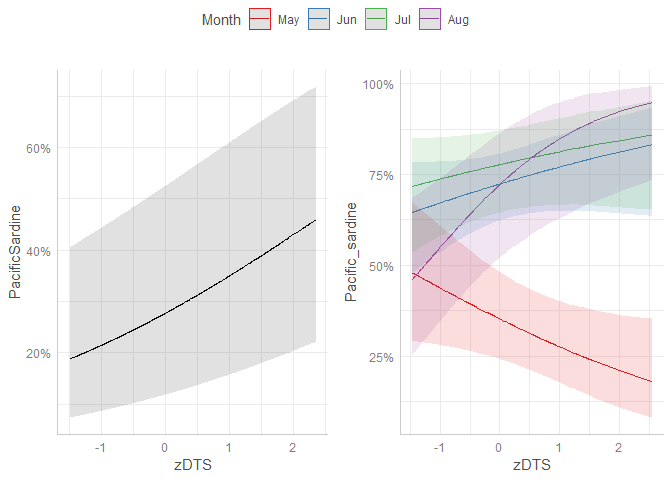
\includegraphics{CPSrevision_files/figure-latex/unnamed-chunk-16-1.pdf}
\caption{predicted probability of Pacific Sardine presence across months
for Shelf (left) and Predator (right) surveys.}
\end{figure}

The effects of salinity in both studies suggested higher presence of
Pacfic sardine with below average salinity.The exception to this pattern
was for samples from May in the predator study which suggest the
presence of sardine increased with \emph{above average} salinity. The
relationship with temperature was really only evident in May samples
from the predator study and indicated higher presence with above average
temperatures. The ws no effect of temperature on Pacific sardine
presence in the shelf study.

\begin{figure}
\centering
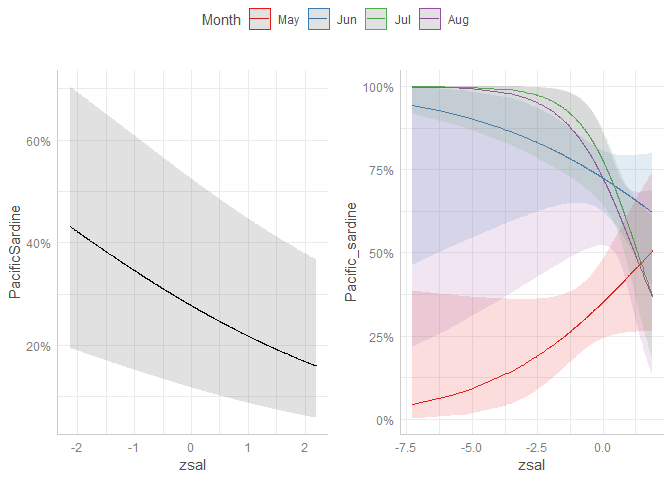
\includegraphics{CPSrevision_files/figure-latex/unnamed-chunk-17-1.pdf}
\caption{predicted probability of Pacific Sardine presence with salinity
for Shelf (left) and across months for the Predator (right) surveys.}
\end{figure}

\begin{figure}
\centering
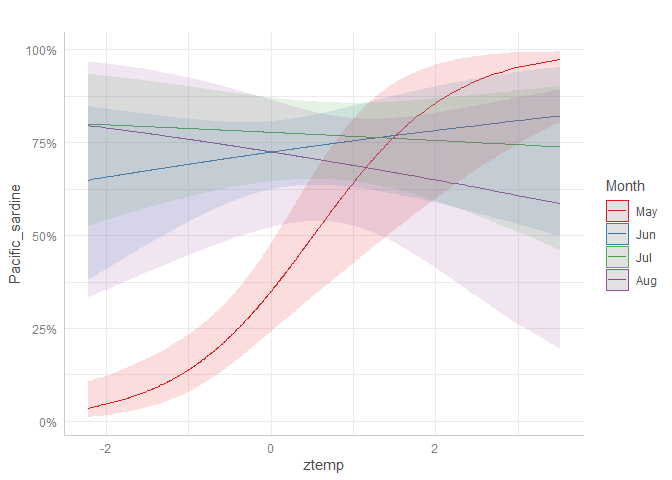
\includegraphics{CPSrevision_files/figure-latex/unnamed-chunk-18-1.pdf}
\caption{predicted probability of Pacific Sardine presence with
temperatureacross months for the Predator (right) surveys.}
\end{figure}

\hypertarget{market-squid-1}{%
\subsubsection{Market Squid}\label{market-squid-1}}

Market squid were encountered in 36\% of all tows in both studies.
Market squid had the highest presence of any CPS species in the shelf
survey. The initial report indicted a strong relationship between Market
Squid presence and both latitude and distance offshore. When splitting
the predator and shelf surveys we found that distance offshore remained
an important factor as did latitude for the shelf survey. In addition,
across both surveys there was an effect of temperature that varied
across months and was generally consistent among the two surveys with
the exception of August.

Distacen offshore was a strong predictor of Market Squid presence in
both surveys. In general, Market Squid presence was predicted to be
higher when tows occurred closer to shore. The effect was particularly
strong during May and June in both surveys. In all other months Market
squid were still predicted to have higher presence closer to shore
though the magnitude of the effect was lower.

\begin{figure}
\centering
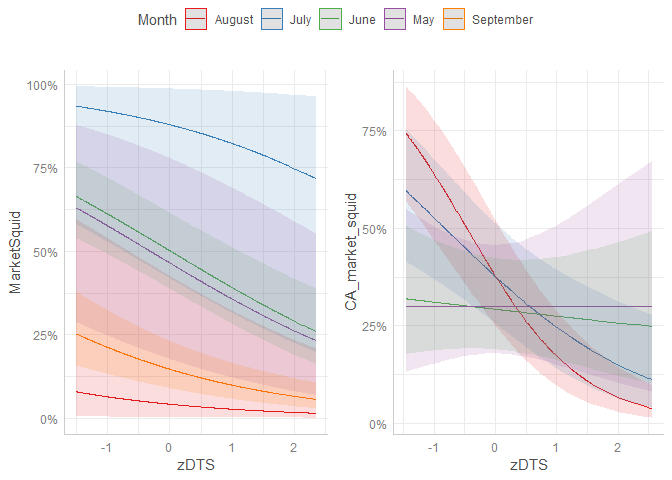
\includegraphics{CPSrevision_files/figure-latex/unnamed-chunk-19-1.pdf}
\caption{predicted probability of Market Squid with distance offshore
across months for Shelf (left) and Predator (right) surveys.}
\end{figure}

Temperature also influenced Market Squid presences across both studies
though the direction of the relationship changed depending on the month
of sampling. Warmer than average temperatures were associated with
higher presence of Market Squid in June and July in both surveys.
Interestingly warmer temps were associated with lower presence of Market
Squid in May. The relationship between Market Squid presence and
temperature during August was positive in the shelf survey and negative
in the predator survey despite temperatures in the same range across
both surveys.

\begin{figure}
\centering
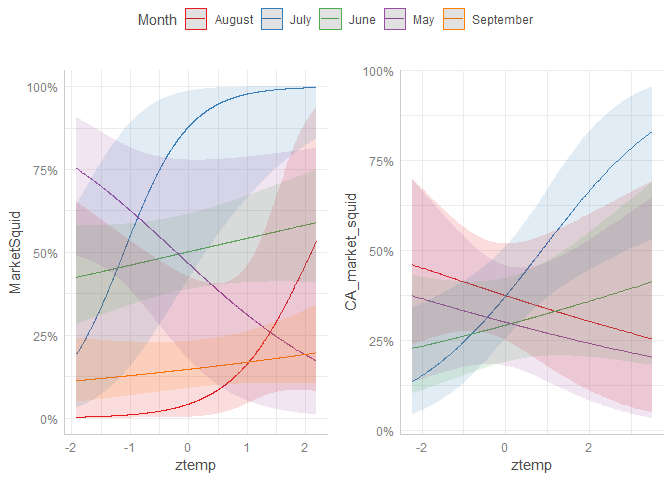
\includegraphics{CPSrevision_files/figure-latex/unnamed-chunk-20-1.pdf}
\caption{predicted probability of Market Squid with temperature across
months for Shelf (left) and Predator (right) surveys.}
\end{figure}

\hypertarget{pacific-mackerel-1}{%
\subsubsection{Pacific Mackerel}\label{pacific-mackerel-1}}

Pacific mackerel were relatively sparse in the predator (17\%) and shelf
(3\%) surveys. Our initial analysis suggested minor effects of
temperature, latitude, and distance offshore. Revised results indicate
that distance offshore and temperature were important for predicting
Pacific mackerel presence in both surveys while there were strogn
monthly differences in predicted presence for the predator survey.
Predicted presence of Pacific mackerel in the predator survey steadily
increased and was significantly different from May through August
ranging from \textasciitilde25 in May to 32\% in August. Our models
predicted higher presence of Pacific mackerel farther offshore.
Similarly, the positive effect of temperature suggested Pacific mackerel
presence increased with warmer than average temps in both studies.
Again, the effects of distance offshore and temperature on Pacific
mackerel presence int he shelf survey described changes in predicted
presence form \textless2\% to \textless5\%.

\begin{verbatim}
## Data were 'prettified'. Consider using `terms="zDTS [all]"` to get smooth plots.
## Data were 'prettified'. Consider using `terms="zDTS [all]"` to get smooth plots.
\end{verbatim}

\begin{figure}
\centering
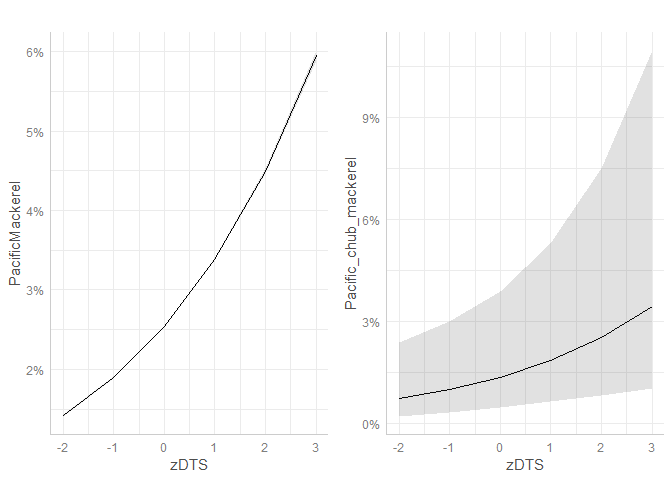
\includegraphics{CPSrevision_files/figure-latex/unnamed-chunk-21-1.pdf}
\caption{predicted probability of Pacific Mackerel with distance
offshore for shelf survey (Left) and predator survey (Right).}
\end{figure}

\begin{verbatim}
## Data were 'prettified'. Consider using `terms="ztemp [all]"` to get smooth plots.
## Data were 'prettified'. Consider using `terms="ztemp [all]"` to get smooth plots.
\end{verbatim}

\begin{figure}
\centering
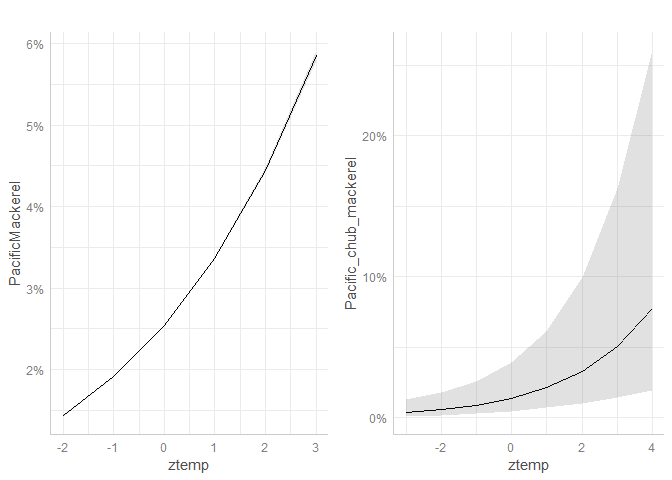
\includegraphics{CPSrevision_files/figure-latex/unnamed-chunk-22-1.pdf}
\caption{predicted probability of Pacific Mackerel with temperature for
shelf survey (Left) and predator survey (Right).}
\end{figure}

\hypertarget{jack-mackerel-1}{%
\subsubsection{\texorpdfstring{\emph{Jack
mackerel}}{Jack mackerel}}\label{jack-mackerel-1}}

Jack mackerel were encountered three times more often in the predator
survey (21\%) than in the shelf survey (7\%). However, our models
provided very little evidence of factors that may influence presence of
the species during our time series. Although the effect of distance to
shore was significant for both datasets, the positive effect was
generally rather weak and did not suggest distance from shore would help
predict presence. However, there was a considerable temporal effect of
month in the predator survey data that indicated a steady and
significant increase in predicted presence of Jack mackerel form May to
August. The model examining the shelf dataset predicted some variability
through the summer but this was largely due to a severe over-prediction
of jack mackerel presence in July.

\begin{figure}
\centering
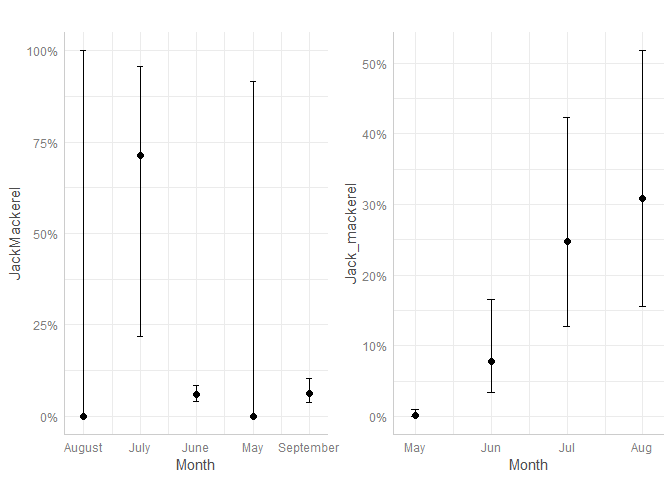
\includegraphics{CPSrevision_files/figure-latex/unnamed-chunk-23-1.pdf}
\caption{predicted probability of Pacific Mackerel by for shelf survey
(Left) and predator survey (Right).}
\end{figure}

\end{document}
